\chapter{Literature Review}

%\section{What is a Literature Review (Temp Section)}
%A lit review...
%
%\begin{itemize}
%	\item surveys related research
%	\item summarizes related research
%	\item links to related research
%\end{itemize}
%
%Gives an indication that I know what is out there, show a sufficient depth of knowledge in the field, and provide context for my research within the broader fields surrounding it.
%
%i.e. the purpose is to...
%
%\begin{itemize}
%	\item define terms / describe theories
%	\item \textbf{justify decisions made}
%	\item what am I building on
%	\item view of alternate approaches / related work
%\end{itemize}
%
%Organise sections by theme. Compartmentalise and synthesise, bringing views and insights together into what is used in the project (good to indicate where in the report it is used). 
%
%Short-ish literature study (20-30\% of manuscript). One to two references for each issue. I must choose well-accredited references. Peer review journal papers and conference papers are preferable. Web pages, forums, tutorials and datasheets are \textit{okay} but not ideal.
%Use reference spreadsheet? Key points, authors, date, title/citation, notes, abstract/relevant snippets.
%
%Topics to cover in this literature review:
%
%\begin{itemize}
%	\item Classification
%	\item Nearest Neighbour (na{\"i}ve benchmark method)
%	\item Multilayer Perceptron (step towards deep learning)
%	\item The concept of 'deep' neural networks - usefulness is using perceptron + convolutional stuff
%	\item Optimization (backpropagation really)
%	\item the MSTAR data set
%	\item image processing (should I be rescaling up or down?)
%	\item direction for expansion (going deeper)
%\end{itemize}
%
%Also need to write a progress report

\section{Synthetic Aperture Radar}
\subsection{Description}
SAR is used to create images of objects, such as vehicles (as in this report), or landscapes. The images are constructed by sending a radar signal from a moving platform, and the time taken for the signal to return to the antenna denotes the size of the aperture. The aperture can be physical, with a large antenna, or synthetic in the case of a moving aperture. Larger apertures allow for higher image resolution. SAR images consist of magnitude and phase data, from which elevation data can be calculated. The classification of 2D SAR images, the type dealt with in this report, requires only the magnitude data to be preserved.
\subsection{Relevance}
The dataset chosen for this report is comprised of SAR imagery. Understanding the nature of the format allows the decision to strip the data of phase information and keep only magnitude data to be made. 

\section{The MSTAR Dataset}
\subsection{Description}
The MSTAR public mixed targets dataset contains X-band synthetic aperture radar (SAR) image chips of multiple targets. Each image has a resolution of 1 foot, and is captured in spotlight mode. Information pertaining to each target, including its elevation, depression angle, and target type is contained in a header section of each file. The header is followed by magnitude and phase data of the SAR imagery. Because the SAR images are 2D, only the magnitude data needs to be considered. Each point represents the brightness of a pixel, reducing the complexity of this study to that of image-based target recognition. \cite{Schumacher_atrof}. Each class of targets has between 195 and 274 instances, with class images ranging in sizes from 48x48 pixels to 198x198 pixels. The targets in each class are rotated between 0\degree and 360\degree.

\subsection{Relevance}
The MSTAR dataset was suggested for this study by A. Mishra. It provides a generic SAR image chip dataset on which any classification method can be run. The dataset is comparatively small, with 195-274 images per class, and thus is suitable for machine learning on a consumer-grade desktop computer with reasonable classification time. The rotation factor present in each image introduces complications, as Figure~\ref{fig:sar_differences} shows, there is a large disparity in appearance between instances of the same class.

\begin{figure}
	\centering
	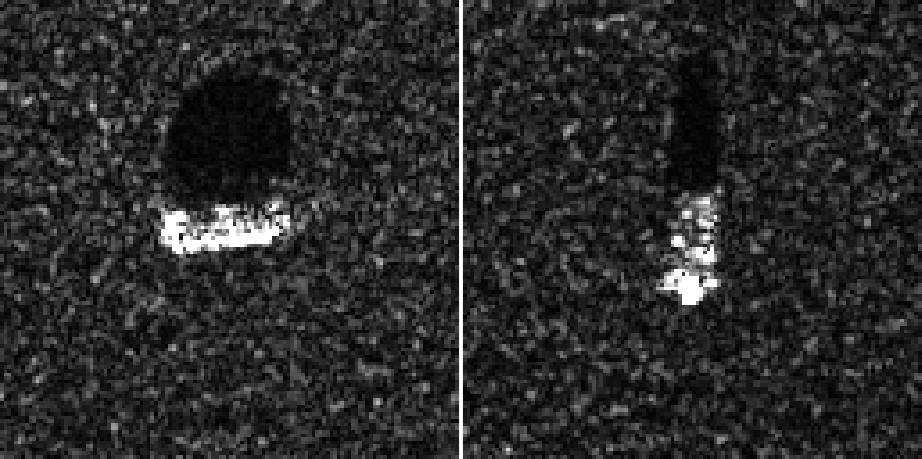
\includegraphics[width=\textwidth]{figures/sar_differences}
	\label{fig:sar_differences}
	\caption{Rotational difference between two images of the same class}
	\centering
\end{figure}



\section{Classification}


\subsection{Nearest-Neighbour Classification}\label{lit:nn}
\subsubsection{Description}
The nearest neighbour classifier operates as follows:
When given an input, the classifier compares this input to the training data set, and finds the one that is closest to the input. For example, if men and women were to be classified by their heights, a given input would be classified as either male or female based on the data point in the training data with the height closest to that of the input. This can be expanded to multiple features/dimensions by taking the Euclidean distance between the input and each instance in the training data set. For images, this amounts to comparing, pixel by pixel, each pixel value, and finding the L2 distance between them. Note that there is no need to apply the square root to the distance; it is a monotonic operation, so it will not affect the ordering of the values, and will introduce additional computational complexity. The equation for calculating the L2 distance is:
\[ d_2(a,b) = (a - b)^2  \]
 Each pixel usually has some relation to the pixels near to it, so there is the possibility for a better definition of 'distance' between images to be made\cite{IMED, Michie94machinelearning}.
 
The nearest neighbour classifier has been shown to provide high classification rates (85+\%) through sufficient image processing and classifier development. A caveat of the success, however, is the inclusion of image chip 'clutter' present in each image affecting the success of clarification. 
Images in the training dataset have similar clutter, and there is a non-negligible contribution to the success of the classification.\cite{Schumacher_atrof}

\subsubsection{Relevance}
The nearest-neighbour classifier is used in this study as an example of a na{\"i}ve classifier. Results of this classifier provide a good benchmark against which subsequent classifier performance can easily be measured. The success of other parties in classifying the MSTAR targets using nearest neighbour methods lays a convincing foundation for future development. There is undoubtedly room for improvement, beginning with the elimination of clutter's effect on classification.


\section{Deep Learning}

The objective of this study is to test the performance of deep learning-based classifiers on SAR image chip data. The success of na{\"i}ve methods has already been proven\cite{Schumacher_atrof}, but lack the predictive power of a truly intelligent classifier. Neural networks and the application of deep learning are key to extracting features from the data to further improve classification rates.

\subsection{Neural Networks}
\subsubsection{Description}
A neural network is a system inspired by the perceived workings of the human brain; a system of neurons combine to perform tasks that exceed their individual capabilities. An input is passed through a series of neuron layers, each of which is tuned to identify characteristic features of the input between each layer, allowing for feature extraction and identification. 

(From the hartford.edu site)
A neural network consists of four main parts\cite{neural_def_russel}:
\begin{enumerate}
	\item Processing units\{uj\}, where each uj has a certain activation level aj(t) at any point in time.
	\item Weighted interconnections between the various processing units which determine how the activation of one unit leads to input for another unit.
	\item An activation rule which acts on the set of input signals at a unit to produce a new output signal, or activation.
	\item Optionally, a learning rule that specifies how to adjust the weights for a given input/output pair.
\end{enumerate}

% must paraphrase or otherwise not plagiarise

\subsubsection{Relevance}
The motivation behind using neural networks is simple; instead of specifying basic characteristics for a system to detect, the system is given an input and a matching output and is left to develop its own perceptions of what important feature link the two. Through optimisation and iteration this can become a very successful form of classification.

\subsection{Multilayer Perceptron}
\subsubsection{Description}
A multilayer perceptron is an extension of the simple perceptron network. The initial design was an input layer, an output layer, and a hidden layer of neurons between. The basic perceptron was deemed unsuitable for complex classification tasks, as its input-output relationship could be reduced (via back-propagation) to a set of linear combinations. This means that is can only correctly classify data that is perfectly linearly separable, which limits its practical applications significantly.

The multilayer perceptron used two or more hidden neuron layers, with non-linear activation functions at each neuron. This makes a multilayer perceptron an example of a deep neural network. The depth allows for more complex feature detection, and ultimately better performance in complex classification tasks. The multilayer perceptron becomes difficult to optimise as the number of hidden layers grows, because the effect of each neuron on the output, and the effects of previous neurons on \textbf{that} neuron become progressively and recursively difficult to compute.
\subsubsection{Relevance}
Implementing a multilayer perceptron is a valuable exercise, as it provides an example of a deep neural network with a fairly straightforward implementation. Training time becomes a significant factor when using a deep neural network due to the time taken to complete back-propagation optimisation, so using a multilayer perceptron will force the development of more efficient methods of data pre-processing to speed up the training as much as possible.

\section{Optimization and Training}
A classifier is only operating efficiently when it is tuned to the data it is attempting to classify. Deep neural networks are initialised with random weights between their neurons, and at first use will perform worse on average than na{\"ive} classification methods. Through optimisation of these inter-neuron weights, however, the potential of deep neural networks can be reached, and classification results are expected to significantly improve. Tuning the classifier to the dataset is crucial, but optimising too heavily may result in \textit{overfitting} of the data, leaving the classifier with no predictive power on unseen data.

% backprop is low-level optimisation, core to the operation
\subsection{Back-propagation}
\subsubsection{Description}
Back-propagation is a system by which the effects of weights between neurons is adjusted through an iterative process. The base case is that of a single input, single output system. 
%I need to put some diagrams in here
Varying the weight on the input directly effects the output. This change can be easily recognised, and the weight can be changed to more suitably link the input to the desired output. This involves developing a method of changing weights in a sensible manner. The most common form of this is through \textit{gradient descent}, whereby the weights are adjusted corresponding to their perceived effect on the output state, and their rate of change. Back-propagation is not guaranteed to find a global minimum, and can settle on a local minimum instead, which can be somewhat alleviated through the use of random weights and multiple training rounds, before choosing the best version of the classifier that has been discovered. 

One of the key issues with back-propagation is its computational complexity. With deep neural networks, the sheer number of weights and their possible combinations make discerning their impact on the output very difficult, and computationally infeasible to perfectly optimise.
%should probably stick a formula in here, but I might save that for the methodology.

\subsubsection{Relevance}
Back-propagation is a popular and successful technique, well-suited to neural networks with only a few layers. With enough time, it can help to optimise much larger networks, and potentially improve classification accuracy by a large margin. It alleviates the concern of trying to find the perfect network from the offset; it allows any network to be tuned to be better than it currently is.

% THERE SHOULD BE SOMETHING ABOUT ACTUAL OPTIMIZATION

\subsection{Hyper-parameters}
\subsubsection{Description}
Hyper-parameters are parameters that, when changed, modify the structure or operation of the neural network, without changing its core mechanics. Hyper-parameters under consideration in this project are:
\begin{itemize}
	\item Image size (100px vs 1000px)
	\item Learning Rate
	\item Network Shape (hidden layer size, and number of layers)
	\item Choice of activation function
	\item Weight initialisations % (sqrt(6)?)
\end{itemize}
\subsubsection{Relevance}


\section{Performance Evaluation}
\subsection{Separability Index}\label{lit:SI}
Thornton's Separability Index (SI) is used as a metric to show how separable the data is into its different classes, i.e. the confidence level with which distinct classes can be identified with no overlap. Perfectly separable data would have an SI of 1, or 100%.

\subsection{Training, Validation, and Testing}\label{lit:loocv}
Successful classification of a dataset is divided into three distinct steps:
\begin{enumerate}
	\item Training
	\item Model Validation
	\item Testing
\end{enumerate}
% http://www-stat.stanford.edu/~tibs/ElemStatLearn/

Training is the process of fitting a classifier - it involves running multiple iterations on a given set of inputs, comparing the output of the classifier to a known target dataset, and adjusting the parameters of the classifier (typically inter-layer weights and bias) through back-propagation. To find the best iteration of the classifier model, it is periodically tested on a different set of known data; the validation dataset. Testing on this intermediate dataset is used to provide performance metrics such as the mean error and the accuracy of classification, which is useful in selecting a model that is optimised to the desired set of parameters. The data from periodically testing on this validation set is used to tune the model, or implement early-stopping procedures. For example, if the desired level of classification accuracy has been achieved or if the mean error hasn't changed significantly after a number of epochs, the training can be stopped early. On the contrary, if the training is approaching its stated limit yet still improving classification accuracy, the number of epochs or 'patience' can be increased to allow for further iterations and tuning.

Once the training is complete, having achieved the desired level of classification accuracy, the chosen model can be tested on another dataset (typically a  set of real-world instances) to see how it performs, providing the testing accuracy. The classifier is no longer tuned, and can be presented with a variety of inputs to simulate its real-world performance.

A dataset is typically split into three sections. 50\% training, 25\% validation, and 25\% testing is a reasonable starting point, and the proportions can be seen as a hyperparameter to be optimised. If the training set is too small, there is a risk that the model will not be able to successfully extract the features required for classification, and its testing accuracy will be low. If the validation or test sets are too small, the model validation and testing might not be thorough enough to cover all reasonable use cases.
% HOW MANY IMAGES IN MSTAR

\subsection{The Confusion Matrix}
%http://www.dataschool.io/simple-guide-to-confusion-matrix-terminology/
% CHECK OUT ROC ANALYSIS AND COHEN's KAPPA
Confusion matrices are useful tools for evaluating classifier performance. They can show the accuracy, misclassification rate, true/false positive rates, specificity, precision, and prevalence. They clearly show the number of correctly classified classes along the matrix's diagonal, and also shows how many of the incorrect classifications were attributed to which classes. 

\section{Hidden Layers}
\section{Logistic Regression}


\section{Dimensionality Reduction}
When dealing with images, the number of pixels grows in proportion to the size of the image. Since every pixel has a weight linking it to the first layer of the neural network, and these weights in turn need to be tuned, the computation power required to train the model is proportional to the size of the input. To reduce computational overhead, it is desirable to reduce the input size, without compromising classification accuracy. This can be done using \textit{dimensionality reduction}.
\subsection{PCA}\label{lit:PCA}

